\documentclass[a4paper]{article}

\usepackage{amssymb,amsmath,amsthm,mathtools}

\usepackage{tikz,hyperref}
\usepackage{graphicx,subfigure}
\usetikzlibrary{spy,calc,patterns,arrows,decorations.pathmorphing,backgrounds,positioning,fit,petri,mindmap,trees,intersections}

%for annotations
\newcommand\annotation[1]{\textcolor{red}{#1}}

%definitions for figures
      \tikzset{neuron/.style = {circle,fill=black!25,minimum size=10pt,inner sep=0pt},
        unit/.style = {neuron, fill=red!50,thick},
    gpu/.style = {rectangle, rounded corners=5pt,draw=green!50, fill=green!20, very thick, minimum width=3.75cm, minimum height = 9.75cm},
        onegpu/.style = {rectangle, rounded corners=5pt,draw=green!50, fill=green!20, very thick, minimum width=17cm, minimum height = 6.5cm},
    pre/.style =    {<-, semithick},
    post/.style =   {->, semithick}
}

\newcommand\DoubleLine[7][1pt]{%
    \path(#2)--(#3)coordinate[at start](h1)coordinate[at end](h2);
    \draw[#4,thick]($(h1)!#1!90:(h2)$)-- node [left=-.75mm] {#5} ($(h2)!#1!-90:(h1)$); 
    \draw[#6,thick]($(h1)!#1!-90:(h2)$)-- node [right=-.75mm] {#7} ($(h2)!#1!90:(h1)$);
    }

%!TEX root = ./master.tex
\theoremstyle{definition}
\newtheorem{calculation}{Calculation}

\title{A Toric Variety from Machine Learning}
\author{Zhangsheng Lai \and Orlando Marigliano}

\begin{document}

\maketitle

%!TEX root = ./master.tex
\section{Introduction}

In this paper, we introduce a new statistical model called the \emph{McCulloch-Pitts process, MPP} which is biologically inspired, for recurrent neural networks....

\section{McCulloch-Pitts Process}

Given a directed graph $G=(V,E)$ with vertex weights $\beta_i > 0$ and edge weights $\alpha_{ij} > 0$, a \emph{McCulloch-Pitts process, MPP} is an activity-based process with binary states $x \in \{0,1\}^{|V|}$ and transitions $xy$ where state $y$ is one-bit away from state $x$. If $y$ and $x$ differs in the $i$-th bit, we define the transition rate 
\begin{align*}
F_{xy} = \left[ \beta_i^{\sigma_i} \alpha_i^{x \sigma_i} \right]^{1/\tau}
\end{align*}


\begin{figure}[h]
\centering
        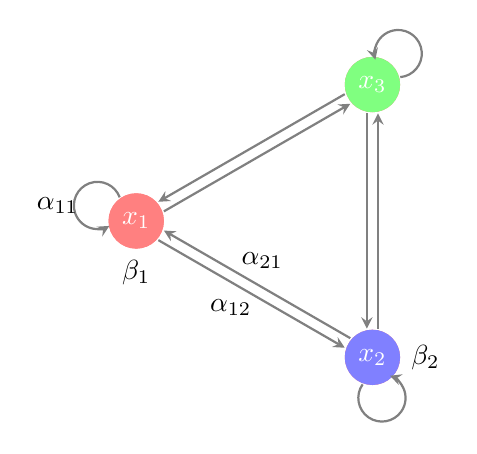
\begin{tikzpicture}[scale = 2,-,draw=black!50, node distance=\layersep,>=stealth]
    \tikzstyle{neuron}=[circle,fill=black!25,minimum size=20pt,inner sep=0pt];
    \tikzstyle{unit1}=[neuron, fill=red!50,thick,];
        \tikzstyle{unit2}=[neuron, fill=blue!50,thick,];
            \tikzstyle{unit3}=[neuron, fill=green!50,thick,];
 \def \radius {1cm}
 \def \n {3}
 \foreach \s in {1,...,\n}{
  \node[unit] (\s) at ({360/\n * (\s - 1) - 180}:\radius) {};
}  
   \DoubleLine{1}{2}{<-,draw=black!50}{}{->,draw=black!50}{};
   \DoubleLine{1}{3}{<-,draw=black!50}{}{->,draw=black!50}{};
    \DoubleLine{2}{3}{<-,draw=black!50}{}{->,draw=black!50}{};
      \node[unit3](k) at ({60}:\radius) {{\color{white}$x_3$}};
  \node[unit1](i) at ({180 }:\radius) {{\color{white}$x_1$}};
    \node[unit2](j) at ({300 }:\radius) {{\color{white}$x_2$}};
    \draw [->,draw=black!50, thick] (1.125) arc (20:300:1.5mm) node[pos=-0.5,left] {} (1);
\draw [->,draw=black!50, thick] (2.250) arc (-215:70:1.5mm) node[pos=-0.5,left] {} (2);
\draw [->,draw=black!50, thick] (3.15) arc (-85:195:1.5mm) node[pos=-0.5,left] {} (3);

    \node[below =.005cm of 1] {$\beta_1$};
%        \node[above left=.05cm of 3] {$\beta_3$};
            \node[right=.005cm of 2] {$\beta_2$};
    \node at (-.4,-.55) {$\alpha_{12}$};
     \node at (-.2,-.25) {$\alpha_{21}$};  
          \node at (-1.5,0.1) {$\alpha_{11}$};    
%\node at (1.255,0.8) {$w_{21}$};
%\node at (2.525,-0.1){$w_{11}$};
\end{tikzpicture}
\caption{McCulloch-Pitts process with three neurons.}
\label{fig:mpp}
\end{figure}

Working with the example in Figure \ref{fig:mpp}, the transition rate matrix is given by

\begin{align*}
    \scalemath{0.7}{
F=\kbordermatrix{
          & 000 & 001 & 010 & 011 & 100 & 101 & 110 & 111 \\
    000 &\ast  & \beta_3 & \beta_2 & 0 & \beta_1 & 0 & 0 & 0 \\
    001 & \beta_3^{-1}\alpha_{33}^{-1} & \ast & 0 & \beta_2\alpha_{32} & 0 & \beta_1\alpha_{31} & 0 & 0  \\
    010 & \beta_2^{-1}\alpha_{22}^{-1} & 0 &\ast  & \beta_3\alpha_{23} & 0 & 0 & \beta_1\alpha_{21} & 0  \\
    011 & 0 & \beta_{2}^{-1}\alpha_{22}^{-1}\alpha_{32}^{-1} & \beta_3^{-1}\alpha_{23}^{-1}\alpha_{33}^{-1} &\ast  & 0 & 0 & 0 & \beta_{1}\alpha_{21}\alpha_{31}  \\
    100 & \beta_1^{-1}\alpha_{11}^{-1} & 0 & 0 & 0 & \ast & \beta_3\alpha_{13} & \beta_{2}\alpha_{12} & 0  \\
    101 & 0 & \beta_1^{-1}\alpha_{11}^{-1}\alpha_{31}^{-1} & 0 & 0 & \beta_{3}^{-1}\alpha_{13}^{-1}\alpha_{33}^{-1} & \ast & 0 & \beta_2\alpha_{12}\alpha_{32}  \\
    110 & 0 & 0 & \beta_1^{-1}\alpha_{11}^{-1}\alpha_{21}^{-1} & 0 & \beta_{2}^{-1}\alpha_{12}^{-1}\alpha_{22}^{-1} & 0 & \ast & \beta_3\alpha_{13}\alpha_{23}  \\
    111 & 0 & 0 & 0 & (\beta_1\alpha_1^{111})^{-1} & 0 & (\beta_2\alpha_{2}^{111})^{-1} & (\beta_3\alpha_{3}^{111})^{-1} & \ast  \\
  }}
\end{align*}

where $\ast$ denotes the negative of the sum of its corresponding row, and $\alpha_i^{111} = \alpha_{1i}\alpha_{2i}\alpha_{3i}$. 

The simulation of the McCulloch-Pitts process starts by drawing an inital state $x^{(0)}$  from a distribution $p^{(0)}$. Then for any state $x$, it holds for some time 
\begin{align*}
\Delta t \sim \text{Exp}(\lambda_x)
\end{align*}
where $\lambda_x = \sum_{y \neq x}F_{xy}$ and it transits to state $y$ which is one hop away with probability 
\begin{align*}
F_{xy}/\lambda_x
\end{align*}
Thus the temporal data obtained from the simulation are binary tuples of length $|V|$ and an associated holding time for each pair of consecutive state.



\section{Toric Variety}
With the statistical model defined proper, we would like to show that the map from the the space of positive parameters $(\beta_i,\alpha_{ij})$ to the space of stochastic rate matrices is a toric map.

\begin{defn}[Toric Map]
ZS to fill up
\end{defn} 

\begin{defn}[Toric Variety]
ZS to fill up
\end{defn} 


Next we would like know the degree and dimension of our toric variety. By first principles, we can obtain them by.... 


{\color{blue}I would like to give some heuristics here, like the degree is the number of interections when we stab the toric variety with a line, plane or in general with a hyperplane. What good does knowing the dimension and degree helps us with and how the method of finding the dimension we used on Wednesday is equivalent to finding the dimension and degree by the method we discuss above.}

%!TEX root = ./master.tex
\section{The Toric Variety}

We consider the space of weights $\mathbb C^{12} = \{(\beta_{i},\alpha_{jk})\mid 1\leq i,j,k\leq 3\}$ and the space of transition rates $\mathbb C^{24} = \{(F_{xy}) \mid x,y \text{ binary states differing at one bit}\}$. We have a map
$f\colon \mathbb C^{12}\to \mathbb C^{24}$ defined by $f(\alpha,\beta) = (F_{xy}(\alpha,\beta))_{xy}$. We define the toric variety $X$ as the Zariski closure of the image of $f$.

Using Polymake, we can compute the Hilbert series of (the closure in $\mathbb P^{24}$ of) $X$. We obtain The Hilbert series
	\[\frac{P(x)}{(1-x)^{12}}\]
with \[P(x)=x^6 + 12x^5 + 51x^4 + 88x^3 + 51x^2 + 12x + 1.\]

The dimension of $X$ is thus $12$, i.\ e.\ the degree of the denominator, and its degree is $P(1)=216$.

\end{document}